\chapter{内存模型}

\section{Java内存模型与线程}
 
\subsection{}

\begin{figure}[H]
    \centering
    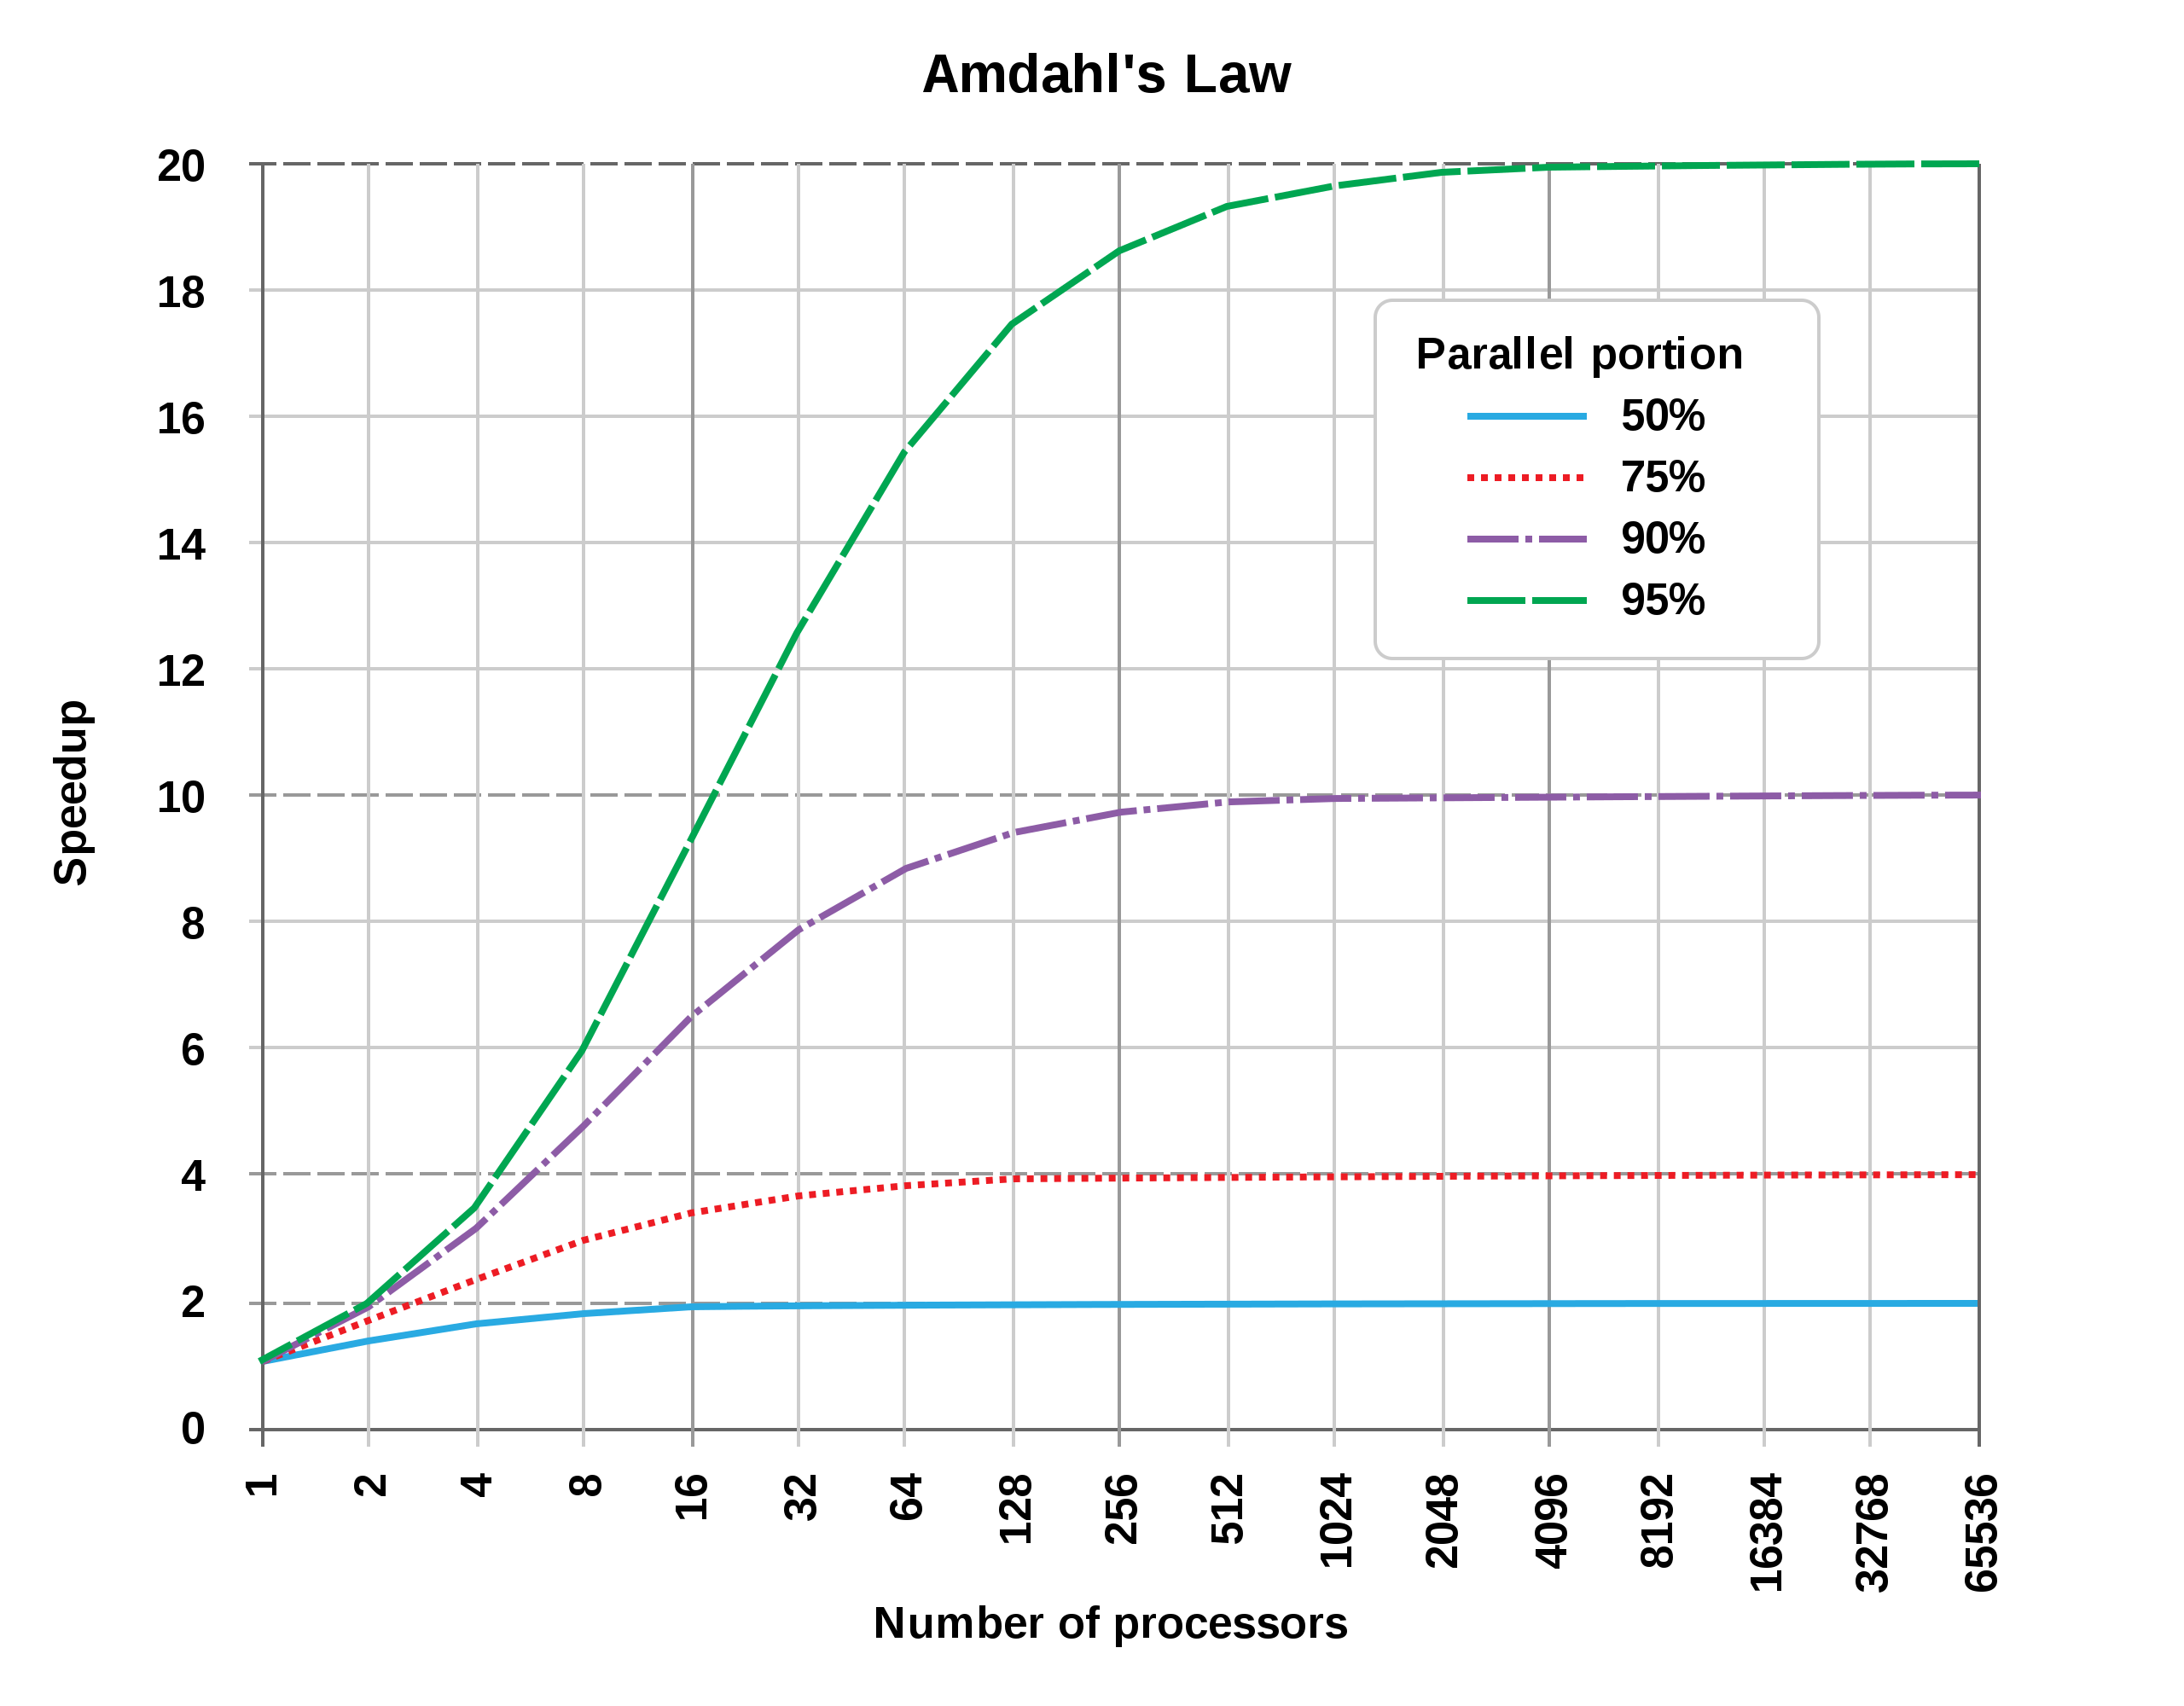
\includegraphics[width=1\textwidth]{parallel/amdahls-law-0.png}
    \caption{Amdahl's Law 阿姆达尔定律}
\end{figure}

并发不得不知的阿姆达定律。

一个程序(或者一个算法)可以按照是否可以被并行化分为下面两个部分:

\begin{itemize}
    \item 可以被并行化的部分
    \item 不可以被并行化的部分 
\end{itemize}


程序串行执行的总时间我们记为\textbf{T}。

时间\textbf{T}包括:不可以被并行和可以被并行部分的时间。不可以并行的部分记为\textbf{B}, 可以被并行的部分就是\textbf{T} - \textbf{B}。即 \textbf{T} = \textbf{B} + (\textbf{T} – \textbf{B}) 

定义如下:

\begin{lstlisting}

 T = 串行执行的总时间

 B = 不可以并行的总时间

 T - B = 并行部分的总时间

\end{lstlisting}


\textbf{T} - \textbf{B} 是可并行化的部分,以并行的方式执行可以提高程序的执行速度。可以提速多少取决于有多少线程或者多少个CPU来执行。线程或者CPU的个数我们记为\textbf{N}。可并行化部分被执行的最快时间可以通过下面的公式计算出来:

(\textbf{T} – \textbf{B} ) / \textbf{N} 或 (1/\textbf{N}) * (\textbf{T} - \textbf{B})

根据阿姆达定律,当可并行部分使用`N`个线程或CPU执行时,程序的总执行时间为:

\textbf{T}(\textbf{N}) = \textbf{B} + (\textbf{T} - \textbf{B}) / \textbf{N}

\notebox{T(N)表示并行因子为N的总执行时间。T(1)就是并行因子为1时的总执行时间。 T(N) = B + (T(1) – B) / N }


示例

\begin{lstlisting}
/*
 * 总时间为1。串行时间为0.4,那么并行时间为0.6。
 */

// 并行因子为2时
T(2) = 0.4 + ( 1 - 0.4 ) / 2
 = 0.4 + 0.6 / 2
 = 0.4 + 0.3
 = 0.7

// 并行因子为5时
 T(5) = 0.4 + ( 1 - 0.4 ) / 5
 = 0.4 + 0.6 / 6
 = 0.4 + 0.12
 = 0.52
\end{lstlisting}

图示

并行因子分别为1,2,3时。

\begin{figure}[H]
    \centering
    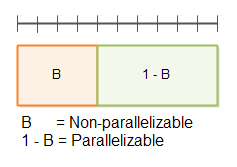
\includegraphics[width=1\textwidth]{parallel/amdahls-law-1.png}
    \caption{并行因子=1}
\end{figure}
\begin{figure}[H]
    \centering
    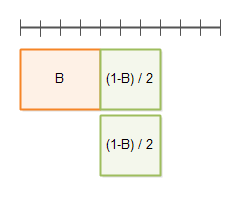
\includegraphics[width=1\textwidth]{parallel/amdahls-law-2.png}
    \caption{并行因子=2}
\end{figure}
\begin{figure}[H]
    \centering
    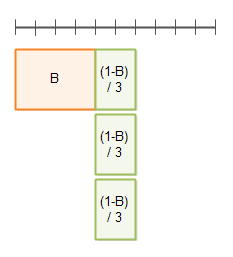
\includegraphics[width=1\textwidth]{parallel/amdahls-law-3.png}
    \caption{并行因子=3}
\end{figure}


\subsubsection{定义} 

并行计算中的\textbf{加速比}是用并行前的执行速度和并行后的执行速度之比来表示的,它表示了在并行化之后的效率提升情况。


 \begin{figure}[H]
    \centering
    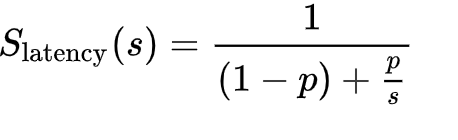
\includegraphics[width=1\textwidth]{parallel/amdahls-definition.png}
    \caption{阿姆达尔定律}
\end{figure}

S(latency)代表理论上的加速比

s 为并行处理结点个数

p 为并行计算部分所占比例

1-p为串行计算部分所占比例

这样:

当p = 1时,最大加速比p = s,

当p = 0时,最小加速比S = 1,

当 s→∞ 时,极限加速比S→ 1/(1-p),这也就是加速比的上限。

例如,若加速前并行代码执行时间占整个代码的执行时间的75%(p=0.75),则加速后并行处理的总体性能的提升不可能超过原先的4倍。

因此可以推断出:

 \begin{figure}[H]
    \centering
    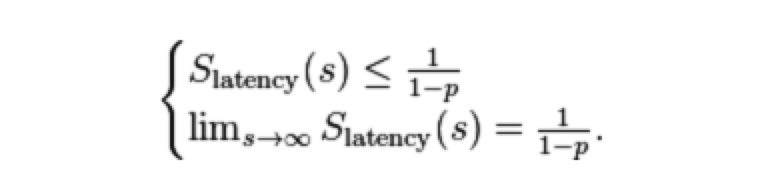
\includegraphics[width=1\textwidth]{parallel/amdahls-definition-1.png}
    \caption{阿姆达尔定律}
\end{figure}

阿姆达尔定律强调:当串行换比例一定时,加速比是有上限的,不管你堆叠多少个CPU参与计算,都不能突破这个上限。


\subsection{Gustafson's law 古斯塔夫森定律}


 \begin{figure}[H]
    \centering
    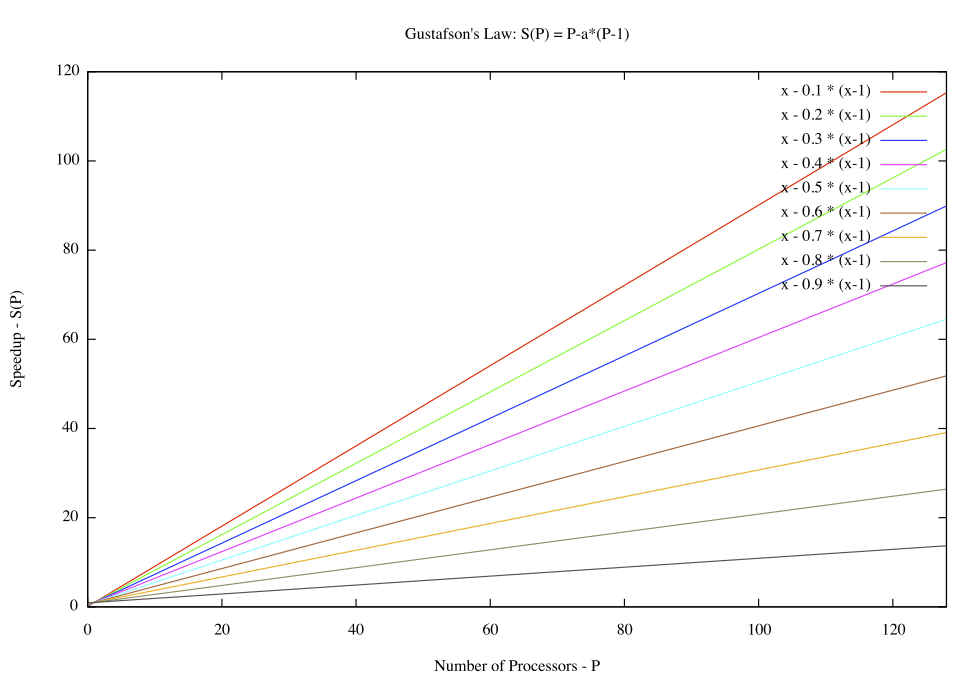
\includegraphics[width=1\textwidth]{parallel/gustafson.png}
    \caption{古斯塔夫森定律}
\end{figure}

 \begin{figure}[H]
    \centering
    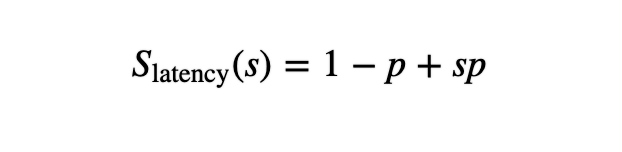
\includegraphics[width=1\textwidth]{parallel/gustafson-definition.png}
    \caption{古斯塔夫森定律定义}
\end{figure}

古斯塔夫森定律强调的是:如果可被并行化的代码所占比例足够大,那么加速比就能随着CPU的数量线性增长。



\subsection{JAVA内存模型 JMM}

JAVA内存模型 Java Memory Model JMM













